\subsection{Thiết kế cơ sở dữ liệu}
\subsubsection{Lược đồ ERD}
\begin{figure}[H]
        \centering
        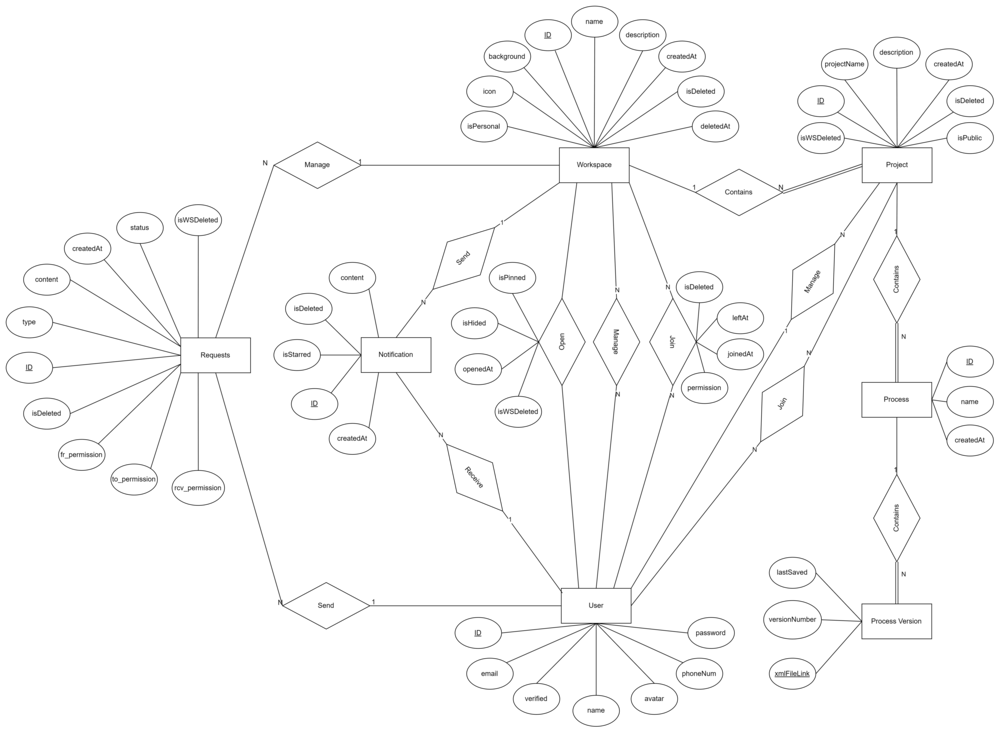
\includegraphics[width=\linewidth]{Content/Phân tích và thiết kế hệ thống/images/erd.png}
        \vspace{0.5cm}
        \caption{Lược đồ ERD}
        \label{fig:Lược đồ ERD}
\end{figure}
\par
Lược đồ ERD gồm có một số thực thể như sau: Workspace, Request,
User, Notification, Project, Process, Process Version với những
thuộc tính như đã được mô tả ở trên. Các thực thể này có một số
quan hệ như sau, và một số quan hệ cũng có những thuộc tính riêng nó:
\begin{itemize}
    \item Một người dùng có thể tham gia nhiều workspace, một
    workspace có thể có nhiều người dùng tham gia.
    \item Một người dùng có thể tạo nhiều request, một request
    chỉ được tạo bởi một người dùng.
    \item Một workspace có thể quản lý nhiều request, một request
    chỉ thuộc về một workspace.
    \item Một người dùng có thể nhận nhiều notification, một
    notification chỉ được gửi bởi một người dùng.
    \item Một người dùng có thể tạo nhiều project, một project
    chỉ được tạo bởi một người dùng.
    \item Một workspace có thể có nhiều project, một project
    chỉ thuộc về một workspace.
    \item Một project có thể có nhiều process, một process
    chỉ thuộc về một project.
    \item Một process có thể có nhiều phiên bản, một phiên bản
    chỉ thuộc về một process.
\end{itemize}

\subsubsection{Ánh xạ ERD và mô tả chi tiết thực thể}
\paragraph{User: Người dùng của hệ thống}
\begin{center}
\begin{tabular}{|p{3cm} |p{2cm} |p{9cm}|}
 \hline
    Thuộc tính & Kiểu & Mô tả \\ [0.5ex] 
 \hline
 \underline{ID} & integer & ID của người dùng. Khoá chính. \\ 
 \hline
 email & varchar & Email của người dùng \\
 \hline
 password & varchar & Mật khẩu của người dùng \\
 \hline
 phoneNumber & varchar & Số điện thoại của người dùng \\
 \hline
 name & text & tên người dùng \\ [1ex] 
 \hline
 avatar & text & Đường dẫn tới ảnh đại diện của người dùng \\
 \hline
 verified & boolean & True nếu tài khoản đã xác thực, False nếu tài khoản chưa xác thực \\
 \hline
\end{tabular}
\end{center}
\begin{figure}[h]
        \centering
        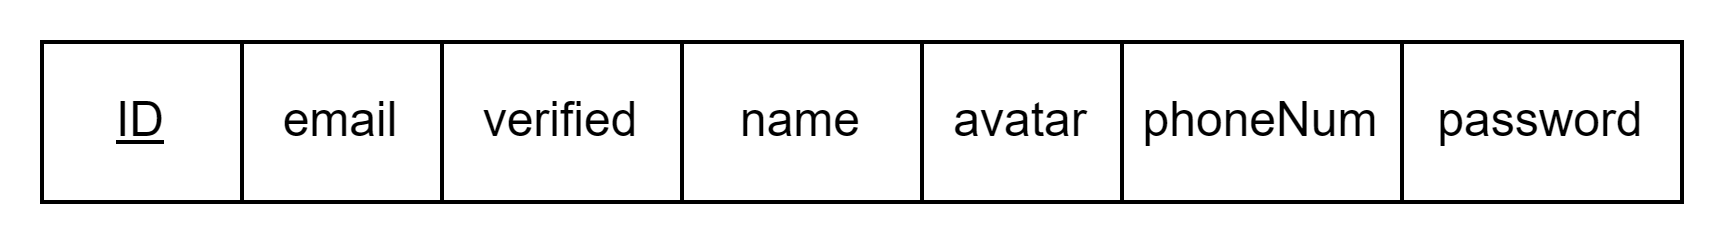
\includegraphics[width=\textwidth]{Content//Phân tích và thiết kế hệ thống//images//ERD_mapping/user_mapping.png}
        \label{fig:enter-label}
\end{figure}
\paragraph{Project: Dự án trong workspace}
\begin{center}
\begin{tabular}{ |p{4cm} |p{3cm} |p{7cm}|} 
 \hline
    Thuộc tính & Kiểu & Mô tả \\ [0.5ex] 
 \hline
 \underline{ID} & integer & ID của project. Khoá chính. \\ 
 \hline
 projectName & text & Tên của project \\
 \hline
 description & text & Mô tả của project \\
 \hline
 isDelete & boolean & Đánh dấu project này đã bị xoá hay chưa \\
 \hline
 createAt & timestamp & Thời gian project được tạo \\
 \hline
 ownerId & integer & ID của người sở hữu project.
 Khoá ngoại tham chiếu tới trường Id trong bảng User \\
 \hline
 workspaceId & integer & ID của workspace nơi mà project được tạo. Khoá ngoại tham chiếu tới trường Id trong bảng Workspace \\
 \hline
 deletedAt & timestamp & Thời gian project được xoá khỏi Workspace \\
 \hline
 isWorkspaceDeleted & boolean & Đánh dấu workspace đã bị xoá hay chưa \\
 \hline
\end{tabular}
\end{center}
\begin{figure}[h]
        \centering
        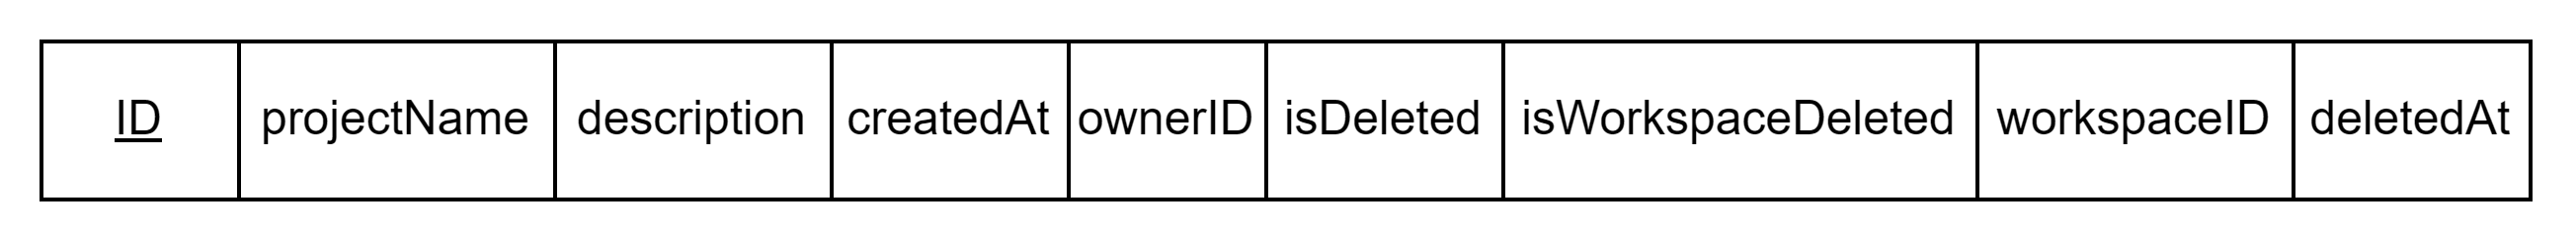
\includegraphics[width=\textwidth]{Content/Phân tích và thiết kế hệ thống/images/ERD_mapping/project_mapping.png}
        \label{fig:enter-label}
\end{figure}

\paragraph{Workspace: Không gian làm việc trong hệ thống}
\begin{center}
\begin{tabular}{ |p{2cm} |p{3cm} |p{9cm}|} 
 \hline
    Thuộc tính & Kiểu & Mô tả \\ [0.5ex] 
 \hline
 \underline{ID} & integer & ID của workspace. Khoá chính. \\ 
 \hline
 name & text & Tên của workspace \\
 \hline
 description & text & Mô tả của workspace \\
 \hline
 isDeleted & boolean & Đánh dấu workspace đã bị xoá hay chưa \\
 \hline
 createAt & timestamp & Thời gian workspace được tạo \\
 \hline
 ownerId & integer & ID của người sở hữu workspace.
 Khoá ngoại tham chiếu tới trường Id trong bảng User \\
 \hline
 background & text & Đường link dẫn tới background của workspace \\
 \hline
 icon & text & Đường link dẫn tới icon của workspace \\
 \hline
 deletedAt & timestamp & Thời gian Workspace được xoá khỏi hệ thống \\
 \hline
 isPersonal & boolean & True nếu đây là workspace cá nhân. False nếu là workspace khác \\
 \hline
\end{tabular}
\end{center}
\begin{figure}[h]
        \centering
        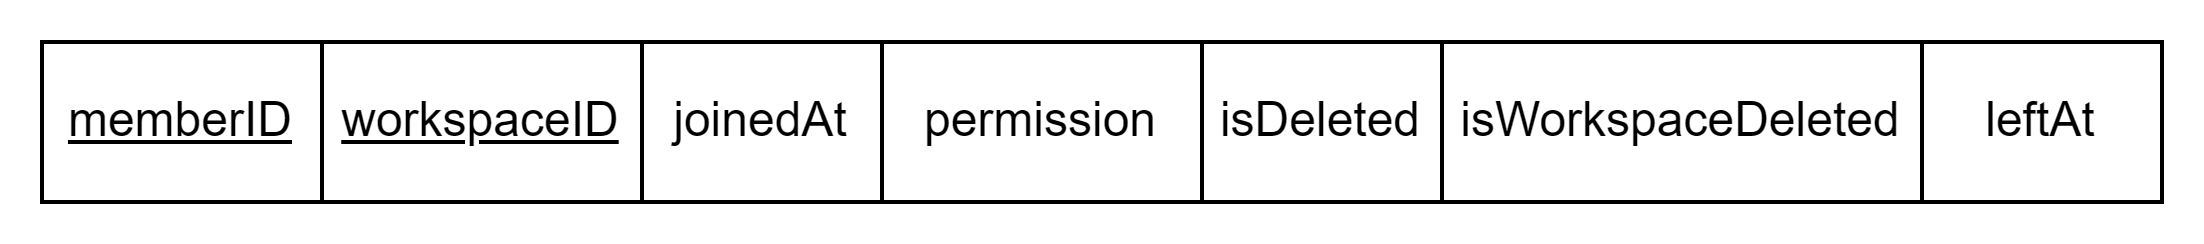
\includegraphics[width=\textwidth]{Content/Phân tích và thiết kế hệ thống/images/ERD_mapping/joinWorkspace_mapping.png}
        \label{fig:enter-label}
\end{figure}

\paragraph{Join Workspace: Quan hệ tham gia giữa người dùng và workspace}
\begin{center}
\begin{tabular}{ |p{3cm} |p{2cm} |p{9cm} |} 
 \hline
    Thuộc tính & Kiểu & Mô tả \\ [0.5ex] 
 \hline
 \underline{memberId} & integer & ID của member tham gia Workspace. Khoá ngoại tham chiếu tới trường Id trong User. \\ 
 \hline
 \underline{workspaceId} & integer & ID của Workspace. Khoá ngoại tham chiếu tới trường Id trong Workspace. \\
 \hline
 joinedAt & timestamp & Thời gian người dùng tham gia Workspace \\
 \hline
 isDeleted & boolean & Đánh dấu người dùng đã rời khỏi Workspace hay chưa \\
 \hline
 permission & text & Quyền hạn của người dùng khi tham gia Workspace \\
 \hline
 leftAt & timestamp & Thời gian người dùng rời khỏi Workspace \\
 \hline
 isWorkspaceDeleted & boolean & Đánh dấu workspace đã bị xoá hay chưa \\
 \hline
\end{tabular}
\end{center}
\begin{figure}[h]
        \centering
        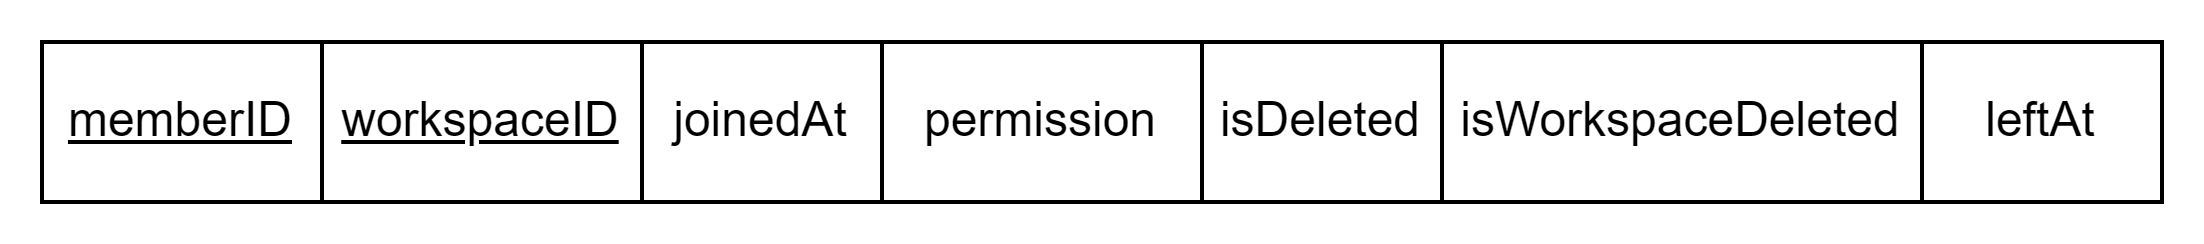
\includegraphics[width=\textwidth]{Content/Phân tích và thiết kế hệ thống/images/ERD_mapping/joinWorkspace_mapping.png}
        \label{fig:enter-label}
\end{figure}

\paragraph{Recent Opened Workspace: Quan hệ chỉnh sửa giữa người dùng và workspace}
\begin{center}
\begin{tabular}{ |p{3cm} |p{2cm} |p{9cm}|} 
 \hline
    Thuộc tính & Kiểu & Mô tả \\ [0.5ex] 
 \hline
 \underline{userId} & integer & ID của member tham gia Workspace. Khoá ngoại tham chiếu tới trường Id trong User. \\ 
 \hline
 \underline{workspaceId} & integer & ID của Workspace. Khoá ngoại tham chiếu tới trường Id trong Workspace. \\
 \hline
 openedAt & timestamp & Thời gian người dùng mở Workspace lần cuối.\\
 \hline
 isHided & boolean & Đánh dấu người dùng đã ẩn Workspace khỏi danh sách của mình hay chưa \\
 \hline
 isPinned & boolean & Đánh dấu người dùng đã pin Workspace vào danh sách ưu tiên hay chưa \\
 \hline
 isWorkspaceDeleted & boolean & Đánh dấu workspace đã bị xoá hay chưa \\
 \hline
\end{tabular}
\end{center}
\begin{figure}[h]
        \centering
        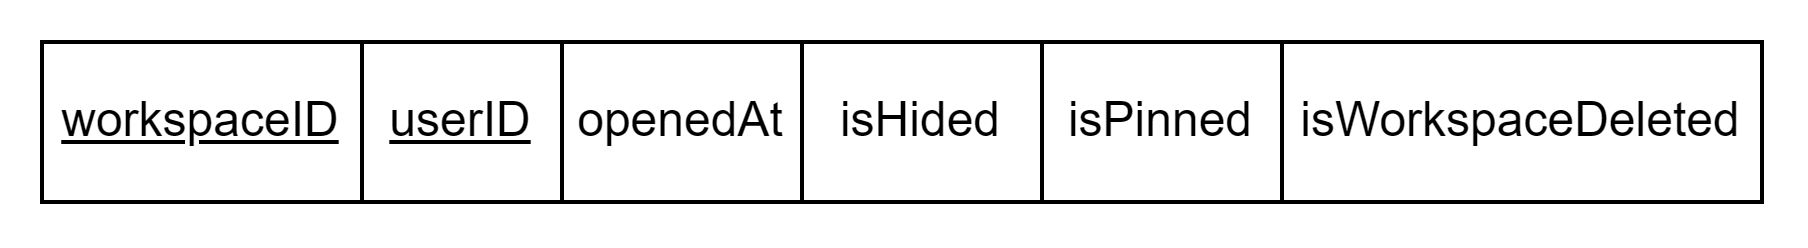
\includegraphics[width=\textwidth]{Content/Phân tích và thiết kế hệ thống/images/ERD_mapping/recent_opened_workspace_mapping.png}
        \label{fig:enter-label}
\end{figure}

\paragraph{Request: Các yêu cầu trong hệ thống}
\begin{center}
\begin{tabular}{ |p{3cm} |p{3cm} |p{9cm}|} 
 \hline
    Thuộc tính & Kiểu & Mô tả \\ [0.5ex] 
 \hline
 \underline{ID} & integer & ID của request. Khoá chính \\ 
 \hline
 type & varchar & Kiểu request \\
 \hline
 createdAt & timestamp & Thời gian người dùng tạo request.\\
 \hline
 status & text & Trạng thái của request, đang được xử lý hay đã được chấp thuận, từ chối.\\
 \hline
 isDeleted & boolean & Đánh dấu request bị xoá hay chưa \\
 \hline
 isWorkspaceDeleted & boolean & Đánh dấu workspace đã bị xoá hay chưa \\
 \hline
 workspaceId & integer & ID của workspace chứa request đó. Khoá ngoại tham chiếu tới trường Id trong Workspace \\
 \hline
  senderId & integer & ID của người gửi request. Khoá ngoại tham chiếu tới trường Id trong User \\
 \hline
  recipientId & integer & ID của người nhận request đã xử lý. Khoá ngoại tham chiếu tới trường Id trong User \\
 \hline
  handlerId & integer & ID của người xử lý request. Khoá ngoại tham chiếu tới trường Id trong User \\
 \hline
  frPermission & text & permission hiện tại của người gửi. \\
 \hline
  toPermission & text & permission mong muốn của người gửi. \\
 \hline
  rcpPermission & text & permission của người sẽ nhận được lời mời tham gia workspace. \\
 \hline
  deletedAt & timestamp & Thời gian xoá request. \\
 \hline
\end{tabular}
\end{center}
\begin{figure}[h]
        \centering
        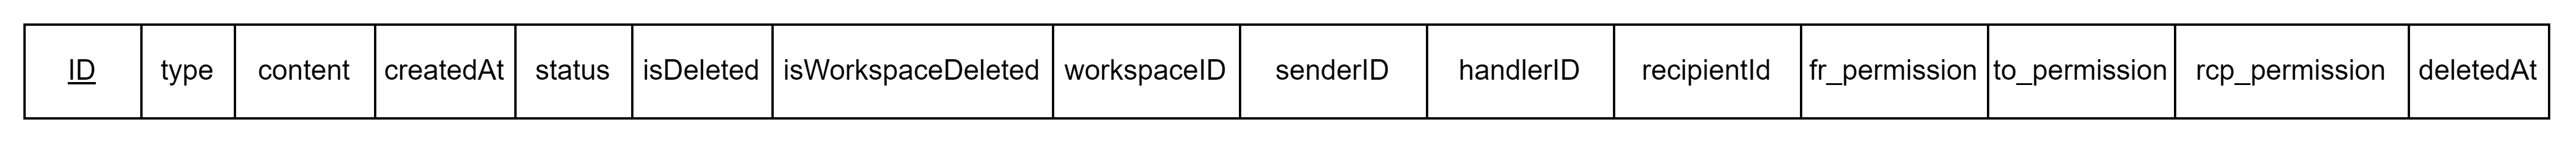
\includegraphics[width=\textwidth]{Content/Phân tích và thiết kế hệ thống/images/ERD_mapping/request_mapping.png}
        \label{fig:enter-label}
\end{figure}

\paragraph{Notification: Các thông báo của người dùng}
\begin{center}
\begin{tabular}{ |p{3cm} |p{3cm} |p{9cm}|} 
 \hline
    Thuộc tính & Kiểu & Mô tả \\ [0.5ex] 
 \hline
 \underline{ID} & integer & ID của thông báo. Khoá chính \\ 
 \hline
 notificationType & varchar & Kiểu thông báo \\
 \hline
 createdAt & timestamp & Thời gian người dùng nhận được thông báo.\\
 \hline
 status & text & Trạng thái của thông báo, đã được chấp thuận hay đồng ý hoặc từ chối lời mời.\\
 \hline
 isDeleted & boolean & Đánh dấu thông báo bị xoá hay chưa \\
 \hline
 isStarred & boolean & Đánh dấu thông báo đã được đánh dấu ưu tiên hay chưa \\
 \hline
 workspaceId & integer & ID của workspace gửi thông báo đó. Khoá ngoại tham chiếu tới trường Id trong Workspace \\
 \hline
  isRead & boolean & Đánh dấu thông báo đã được đọc hay chưa \\
 \hline
  permission & text & permission của người nhận. \\
 \hline
  deletedAt & timestamp & Thời gian xoá request. \\
 \hline
\end{tabular}
\end{center}
\begin{figure}[h]
        \centering
        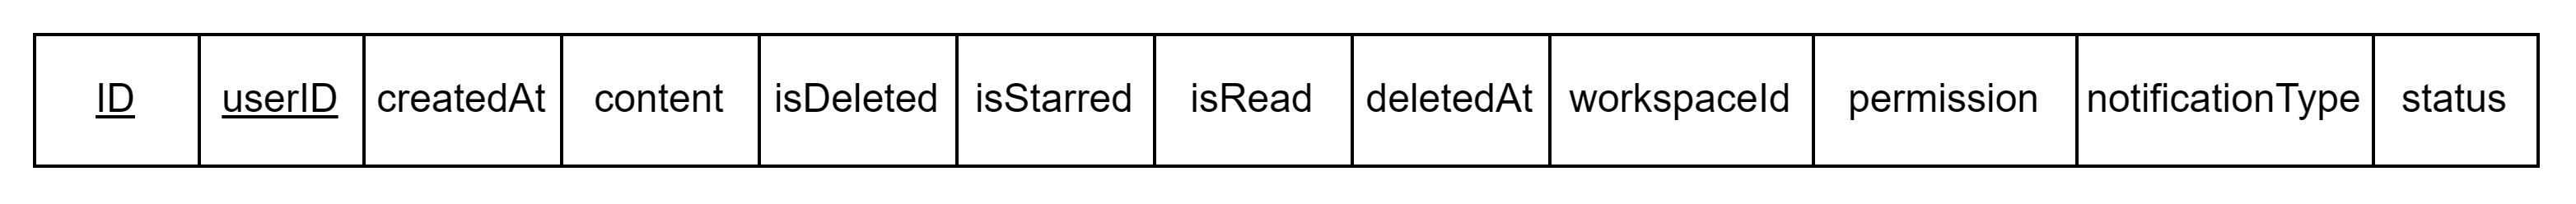
\includegraphics[width=\textwidth]{Content/Phân tích và thiết kế hệ thống/images/ERD_mapping/notification_mapping.png}
        \label{fig:enter-label}
\end{figure}